\chapter{The Frontend Application}
\label{frontend}
	\section{Introduction}
		\begin{figure}[H]
			\iftrue
			\caption{Frontend Application}
			\centering
			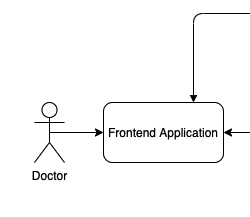
\includegraphics[scale=0.5]{figures/frontend}
			\fi
		\end{figure}
		In this chapter we will have a look at the technology stack, internals and points of interest of the frontend application. The
		frontend applications purpose is to serve as a visual middleware between the end-user (The Doctor) and the system itself. It 
		propagates the actions of the user into the system by using plain HTTPS Requests, via a stateful[\cite{session-rfc6265}],
		Json-based[\cite{json-rfc7159}] Https[\cite{rfc2818}] RESTFull[\cite{restful-rfc7231}]
		protocol (for more information please see chapter \ref{API}).
	\section{Technology Stack}
		The Frontend application uses the following frameworks and libraries
		\begin{itemize}
			\item React v18.0
			\item Boostrap v4
			\item Axios Requests
			\item Hansontable v8.3.2
		\end{itemize}
		\subsection{React}
			React.js is an javascript open-source framework for developing front-end applications. It is created by Facebook and 
			maintained by the open-source communinity as well as from some individual companies. It encourages the creation applicatios
			with well defined state and state transisions by composing lightweight and reusable UI Elements called 'Components'. The
			behaviour of the system is modelled strictly by events generated as a result of a state transision and the components should
			act accordingly. Our Frontend Application contains 13 indepedent components that communicate with each other by callbacks.
			An exchaustive list of the components is given below
			\begin{center}
				\begin{tabular}{ |c|c|c| } 
					\hline
					About & The About page &
\includegraphics[scale=0.2]{figures/component-about}\\
					About & The About page &
\includegraphics[scale=0.2]{figures/component-about}\\
					About & The About page &
\includegraphics[scale=0.2]{figures/component-about}\\
					About & The About page &
\includegraphics[scale=0.2]{figures/component-about}\\
					About & The About page &
\includegraphics[scale=0.2]{figures/component-about}\\
					About & The About page &
\includegraphics[scale=0.2]{figures/component-about}\\
					About & The About page &
\includegraphics[scale=0.2]{figures/component-about}\\
					About & The About page &
\includegraphics[scale=0.2]{figures/component-about}\\
					About & The About page &
\includegraphics[scale=0.2]{figures/component-about}\\
					About & The About page &
\includegraphics[scale=0.2]{figures/component-about}\\
					About & The About page &
\includegraphics[scale=0.2]{figures/component-about}\\
					About & The About page &
\includegraphics[scale=0.2]{figures/component-about}\\
					About & The About page &
\includegraphics[scale=0.2]{figures/component-about}\\
					\hline
				\end{tabular}
			\end{center}
			